%% 
%% Copyright 2019-2024 Elsevier Ltd
%% 
%% Manuscript for Control Engineering Practice (Elsevier / IFAC)
%% Using CAS double column class (cas-dc.cls)
%% 
\documentclass[a4paper,fleqn]{cas-dc}

\usepackage[numbers]{natbib}
\usepackage{amsmath,amssymb,amsfonts}
\usepackage{booktabs}
\usepackage{graphicx}
\graphicspath{{figuras/}{../figuras/}}
\usepackage{array}
\usepackage{multirow}
\usepackage{url}
\usepackage{xcolor}

%%% Author macros
\def\tsc#1{\csdef{#1}{\textsc{\lowercase{#1}}\xspace}}
\tsc{WGM}
\tsc{QE}

\begin{document}
\let\WriteBookmarks\relax
\def\floatpagepagefraction{1}
\def\textpagefraction{.001}

% Short title & short authors
\shorttitle{Model Predictive DVFS for Spaceborne AI Clusters in Orbital Vacuum}    
\shortauthors{D. T. C. M. Barros and F. B. Braz da Silva}  

% Main title
\title[mode = title]{Thermal-Crosstalk-Aware Scheduling and Model Predictive Dynamic Voltage and Frequency Scaling for Spaceborne Multi-Chip AI Clusters in Deep Vacuum}  

% Author 1: Dafnhe Barros
\author[1]{Dafnh\^e~T.~C.~M.~Barros}[orcid=0009-0004-9840-0257]
\cormark[1]
\ead{dafnhe.barros@msn.com}
\credit{Conceptualization, Methodology, Software, Validation, Formal analysis, Investigation, Data curation, Writing - original draft}

% Author 2: Flavio Braz da Silva
\author[1]{Fl\'avio~B.~Braz~da~Silva}[orcid=0000-0002-4752-9742]
\ead{flavio.silva@ifes.edu.br}
\credit{Supervision, Project administration, Resources, Writing - review \& editing}

% Affiliation
\affiliation[1]{organization={Graduate Program in Control and Automation Engineering (ProPECAut), Federal Institute of Esp\'irito Santo (IFES)},
            addressline={Rodovia BR-101 Norte, Km 58}, 
            city={Serra}, 
            postcode={29166-064}, 
            state={Esp\'irito Santo}, 
            country={Brazil}}

\cortext[1]{Corresponding author.}

% Highlights (3-5 points, max 85 characters per point)
\begin{highlights}
\item Non-linear $5\times5$ compact thermal modeling and EKF state estimation in deep vacuum.
\item Constrained discrete LTV MPC-DVFS via warm-started ADMM for crosstalk control.
\item Radiative power budgeting under solar radiation, Earth albedo, and eclipse forecast.
\item 3-orbit LEO co-simulation achieves zero observed thermal violations and 77.6\% gradient drop.
\item Latin Hypercube Sampling ($n=30$) evaluates thermal sensitivity under uncertainty.
\end{highlights}

% Abstract
\begin{abstract}
High-density heterogeneous artificial intelligence (AI) computing clusters onboard small satellites in Low Earth Orbit (LEO) face severe electrothermal constraints. Gas-mediated convective heat transfer is neglected in the adopted high-vacuum model ($h \approx 0$), confining thermal rejection exclusively to internal solid conduction and non-linear Stefan-Boltzmann radiation to deep space ($q \propto T^4$). In multi-chip modules (MCM), heavy neural inference workloads induce severe lateral conductive coupling between adjacent silicon dies (\textit{thermal crosstalk}). This paper investigates a model-based predictive thermal management strategy, denoted \textbf{TCAS-DVFS} (\textit{Thermal-Crosstalk-Aware Scheduling and Model Predictive Dynamic Voltage and Frequency Scaling}), formulated from lumped thermodynamic principles for multi-die spaceborne accelerators. The proposed architecture integrates: (i) real-time state estimation via an Extended Kalman Filter (EKF) operating over a non-linear $5\times5$ Compact Thermal Model (CTM); (ii) a discrete linear time-varying Model Predictive Controller (LTV MPC-DVFS) that solves a condensed quadratic program via a warm-started ADMM-style splitting iteration, coordinating operating frequencies; (iii) a dynamic temperature-referenced radiative power-budget surrogate derived from orbital ephemerides and ambient flux forecasts; and (iv) a topological task allocator relaxed over the semidefinite cone $\mathbb{S}_+^{17}$ via Semidefinite Programming (SDP). In a three-orbit numerical co-simulation of a 500-km circular LEO scenario (17,004.0~s, 34,009 time samples, 4 processing dies), TCAS-DVFS produced zero observed junction temperature violations above the 85~$^\circ$C threshold ($0\text{ s}$ versus 200.5~s for binary Thermal Throttling at 85/75~$^\circ$C and 14.0~s for Space-PID), attenuated peak inter-die thermal gradients by 77.6\% (reducing from 9.42 to 2.11~K), and maintained an aggregate throughput of 124.38~FPS with an energy-delay product proxy ($E_{t_{\mathrm{frame}}}$) of 7.477~kJ$\cdot$s/frame. Functional ablation indicates a dominant contribution from the predictive control formulation in damping gradients and bounding temperatures, whereas topological SDP scheduling provides limited observed benefits in compact arrangements ($N=4$ dies) due to conductive symmetry. Sensitivity was evaluated under a 30-sample Latin Hypercube Sampling (LHS) stress-test envelope ($\pm20\%$ parameter variation), yielding zero observed violations with an exact 95\% Clopper-Pearson upper confidence bound of 11.57\%, where die-to-radiator thermal resistance ($R_r$) exhibited the strongest monotonic association with $T_{\max}$ (Spearman $\rho = +0.994$). Indicative reliability proxy analyses demonstrate that electromigration yields no life extension (relative Black damage ratios of 0.96 and 0.81), whereas cyclic thermal stress severity is noticeably damped. The reported evidence is limited to numerical simulation of the stated lumped-parameter model and does not constitute hardware or flight qualification.
\end{abstract}

\begin{keywords}
Control applications \sep Model predictive control \sep Thermal crosstalk \sep Dynamic voltage and frequency scaling \sep Spaceborne computing \sep Orbital vacuum thermodynamics
\end{keywords}

\maketitle

\section{Introduction}
\label{sec:intro}

\subsection{Orbital Edge Computing and Spaceborne AI}
Modern Earth Observation (EO) satellite missions, including wildfire monitoring, maritime surveillance, disaster response, and Synthetic Aperture Radar (SAR) imaging, produce massive data streams operating at multi-gigabit-per-second rates in Low Earth Orbit (LEO)~\citep{denby2020asplos, garrett2024taes, chen2026sagin}. Traditionally, remote sensing platforms have relied on the conventional \textit{store-and-forward} architecture, wherein raw payload data are captured, buffered in solid-state recorders, and downlinked during brief 8-to-12-minute ground-station passes per orbit. This approach incurs severe latency penalties, frequently exceeding 4 to 12 hours~\citep{denby2020asplos, garrett2024taes}.

Edge artificial intelligence (AI) onboard small satellites mitigates this downlink bottleneck by processing, compressing, and triaging sensor data directly in orbit using commercial off-the-shelf (COTS) neural accelerators, multicore ARM CPUs, and embedded GPUs~\citep{garrett2024taes, sherwood2003ase}. In particular, automated on-orbit cloud segmentation enables the autonomous discarding of up to 67\% of optically obstructed imagery prior to transmission~\citep{king2013spatial}, thereby conserving scarce communication bandwidth for high-priority mission products~\citep{giuffrida2021phisat1}.

\subsection{Deep Vacuum Thermodynamics and Thermal Crosstalk}
Unlike terrestrial data centers that leverage forced air convection ($h \approx 20$--$100\text{ W/(m}^2\text{K)}$) or pumped liquid cooling loops ($h \approx 1,000$--$10,000\text{ W/(m}^2\text{K)}$)~\citep{incropera2011fundamentals}, small spacecraft operating in the high vacuum of LEO ($P < 10^{-4}\text{ Pa}$, free molecular flow with Knudsen number $Kn \gg 10$)~\citep{gilmore2002handbook} exhibit negligible convective gas exchange. Consequently, gas-mediated convective heat transfer is neglected in the adopted high-vacuum model ($h \approx 0$). Thermal rejection from energized silicon junctions is restricted to two coupled mechanisms~\citep{ecss2008thermal, gilmore2002handbook}:
\begin{enumerate}
\item \textbf{Internal solid conduction:} heat dissipates from active junctions across thermal interface materials (TIM) into a shared cold plate or metallic carrier (e.g., AlN or Al 6061-T6, $k \approx 170\text{--}200\text{ W/(m}\cdot\text{K)}$)~\citep{ecss2008thermal}. Direct radiative exchange between facing die side-walls is negligible ($< 10^{-3}\text{ W}$ due to microscopic lateral areas $A_{lat} \approx 10^{-5}\text{ m}^2$ and small temperature differences).
\item \textbf{External radiation to deep space:} structural heat reaches outer passive radiators and is radiated to the cold cosmic background ($T_{space} \approx 2.73\text{ K}$) governed by the non-linear Stefan-Boltzmann law ($q_{rad} \propto \varepsilon \sigma T^4$)~\citep{incropera2011fundamentals, pederson2024radiator}.
\end{enumerate}

In compact small-satellite form factors (e.g., 6U--12U CubeSats), volume and mass constraints dictate packaging multiple System-on-Module (SoM) accelerators on a single carrier. Simultaneous deep neural inference workloads dissipate between 10 and 25~W per die~\citep{reuther2022accelerator, kang2025power}, demanding 60 to 100~W from the electrical power system (EPS). Crucially, lateral conductive flux propagating through the carrier raises the base temperature of neighboring idle or lightly loaded dies by 10 to 18~K within tens of seconds~\citep{chen2026hotai, wang2025packaging}. This mutual conductive coupling, termed \textbf{spatial thermal crosstalk}, induces mutual thermal interference and severely degrades uncoordinated, decentralized governors.

\subsection{Deficiencies of Terrestrial Thermal Governors}
Conventional reactive algorithms, such as the Linux \textit{ondemand} governor~\citep{pallipadi2006ondemand} and classical Single-Input Single-Output (SISO) PID loops, fail in orbital clusters due to three structural factors~\citep{brooks2001dtm, skadron2004hotspot, hoffmann2021online}:
\begin{enumerate}
\item \textbf{Large thermal inertia:} passive radiators ($C_{rad} \approx 1,300\text{ J/K}$) introduce dominant time constants of tens of minutes, causing purely reactive policies to act with critical delay.
\item \textbf{Limit-cycle saw-tooth oscillations:} binary frequency throttling upon crossing emergency alarm thresholds triggers repetitive temperature fluctuations ($\Delta T \approx 10\text{ K}$).
\item \textbf{Spatial gradient amplification:} uncoordinated DVFS across asymmetric workloads exacerbates instantaneous temperature differentials across adjacent dies, accelerating low-cycle thermomechanical shear fatigue in Ball Grid Array (BGA) solder interconnects~\citep{manson1966fatigue}.
\end{enumerate}

\subsection{Research Question and Contributions}
The pioneering work of \citet{chen2026hotai} established thermal-crosstalk-aware task scheduling in spaceborne AI clusters. Building on this domain, our work investigates the following research question:
\begin{quote}
\textit{Can a model-based coordinated MPC-DVFS policy reduce thermal-threshold exceedance and inter-die temperature gradients in a simulated four-die orbital AI cluster while maintaining competitive inference throughput relative to reactive thermal governors under identical modeled workload and environmental conditions?}
\end{quote}
To address this question through model-based numerical simulation, this paper presents the following contributions and findings within the scope of the modeled multi-physics system:
\begin{enumerate}
\item \textbf{Non-linear State-Space Electrothermal Modeling:} we formulate a $5\times5$ compact thermal network (CTM) capturing conductive coupling matrices, linearized Stefan-Boltzmann radiator dynamics, and non-linear subthreshold leakage positive feedback, integrated with an Extended Kalman Filter (EKF) observer under stochastic sensor noise.
\item \textbf{Constrained Predictive Control (LTV MPC-DVFS):} we formulate a discrete linear time-varying Model Predictive Controller that solves a condensed quadratic programming problem via a warm-started ADMM-style splitting iteration, coordinating operating frequencies to track inference workloads, enforce a nominal 83~$^\circ$C limit, and suppress spatial gradients.
\item \textbf{Orbital Radiative Power Budget Surrogate:} we derive a predictive moving-average budget for solar flux, terrestrial albedo, and Earth infrared radiation to establish a temperature-referenced power envelope under eclipse transitions.
\item \textbf{Numerical Robustness and Methodological Demarcation:} we execute a three-orbit numerical co-simulation, functional ablation, a 30-sample Latin Hypercube Sampling (LHS) stress-test campaign with exact Clopper-Pearson coverage bounds, and physics-of-failure reliability proxy evaluations.
\end{enumerate}

To ensure complete methodological transparency, Table~\ref{tab:demarcacao} establishes the explicit demarcation between input assumptions, synthetic drivers, calculated simulation states, evaluated proxies, and physically unmeasured quantities.

\begin{table*}[t]
\caption{Methodological Demarcation of Study Elements}
\label{tab:demarcacao}
\centering
\small
\begin{tabular*}{\textwidth}{@{\extracolsep{\fill}}lp{0.72\textwidth}@{}}
\toprule
\textbf{Methodological Category} & \textbf{Specific Elements in this Study} \\
\midrule
Input Physical Parameters & Conductive resistances $R_{ij}$, die-to-radiator resistance $R_r$, die capacitances $c_i$, radiator capacitance $C_{rad}$, optical emissivity $\varepsilon$, solar absorptivity $\alpha_s$ (Table~\ref{tab:params}) \\
Model Hypotheses \& Structure & Lumped-parameter $5\times5$ CTM; gas conduction neglected ($h \approx 0$); linearized radiative state coupling; planar symmetry \\
Synthetic Workload Inputs & Continuous activity factors $\alpha_i(t)$ and nominal requested frequencies $f_{nom,i}(t)$ across 4 mission workloads \\
Model Environmental Forcing & Direct solar flux $Q_{sol}(t)$, Earth albedo $Q_{alb}(t)$, and terrestrial infrared $Q_{IR}(t)$ across a 500-km circular orbit \\
Calculated State Variables & Physical silicon junction temperatures $T_i(t)$ ($i=1,\dots,4$) and radiator core temperature $T_{rad}(t)$ \\
Estimated State Variables & EKF state estimates $\hat{T}_i(t)$ and $\hat{T}_{rad}(t)$ reconstructed from noisy sensor measurements ($\sigma_s = 0.25\text{ K}$) \\
Actuation Control Variables & Operating clock frequencies $\mathbf{f}(t) = [f_1(t), \dots, f_4(t)]^T \in [0.30, 1.30]\text{ GHz}$ \\
Direct Numerical Outputs & Maximum temperature $T_{\max}$, spatial gradient $\Delta T_{esp}(t)$, violation time $t_{>85}$, total energy $E$ \\
Evaluated Computational Proxies & Aggregate throughput proxy $\mathrm{FPS}$, energy-delay product proxy $E_{t_{\mathrm{frame}}}$, relative Black electromigration damage ratio, thermal-history rainflow cycle distribution \\
Unmeasured Physical Quantities & Physical component service life, BGA viscoplastic solder strain, internal package micro-gradients, space radiation effects (TID/SEE), and flight qualification \\
\bottomrule
\end{tabular*}
\end{table*}

The remainder of this article is organized as follows: Section~\ref{sec:env} presents the orbital environmental physics and radiative balance. Section~\ref{sec:model} derives the electrothermal state-space model. Section~\ref{sec:control} develops the TCAS-DVFS control architecture. Section~\ref{sec:sim_method} details the co-simulation methodology. Section~\ref{sec:results} presents comparative simulation results, ablation, and parametric sensitivity. Section~\ref{sec:reliability} evaluates indicative reliability proxies. Section~\ref{sec:related} discusses related work, Section~\ref{sec:practice} discusses practical implementation considerations and threats to validity, and Section~\ref{sec:concl} concludes the paper.

\begin{figure}
\centering
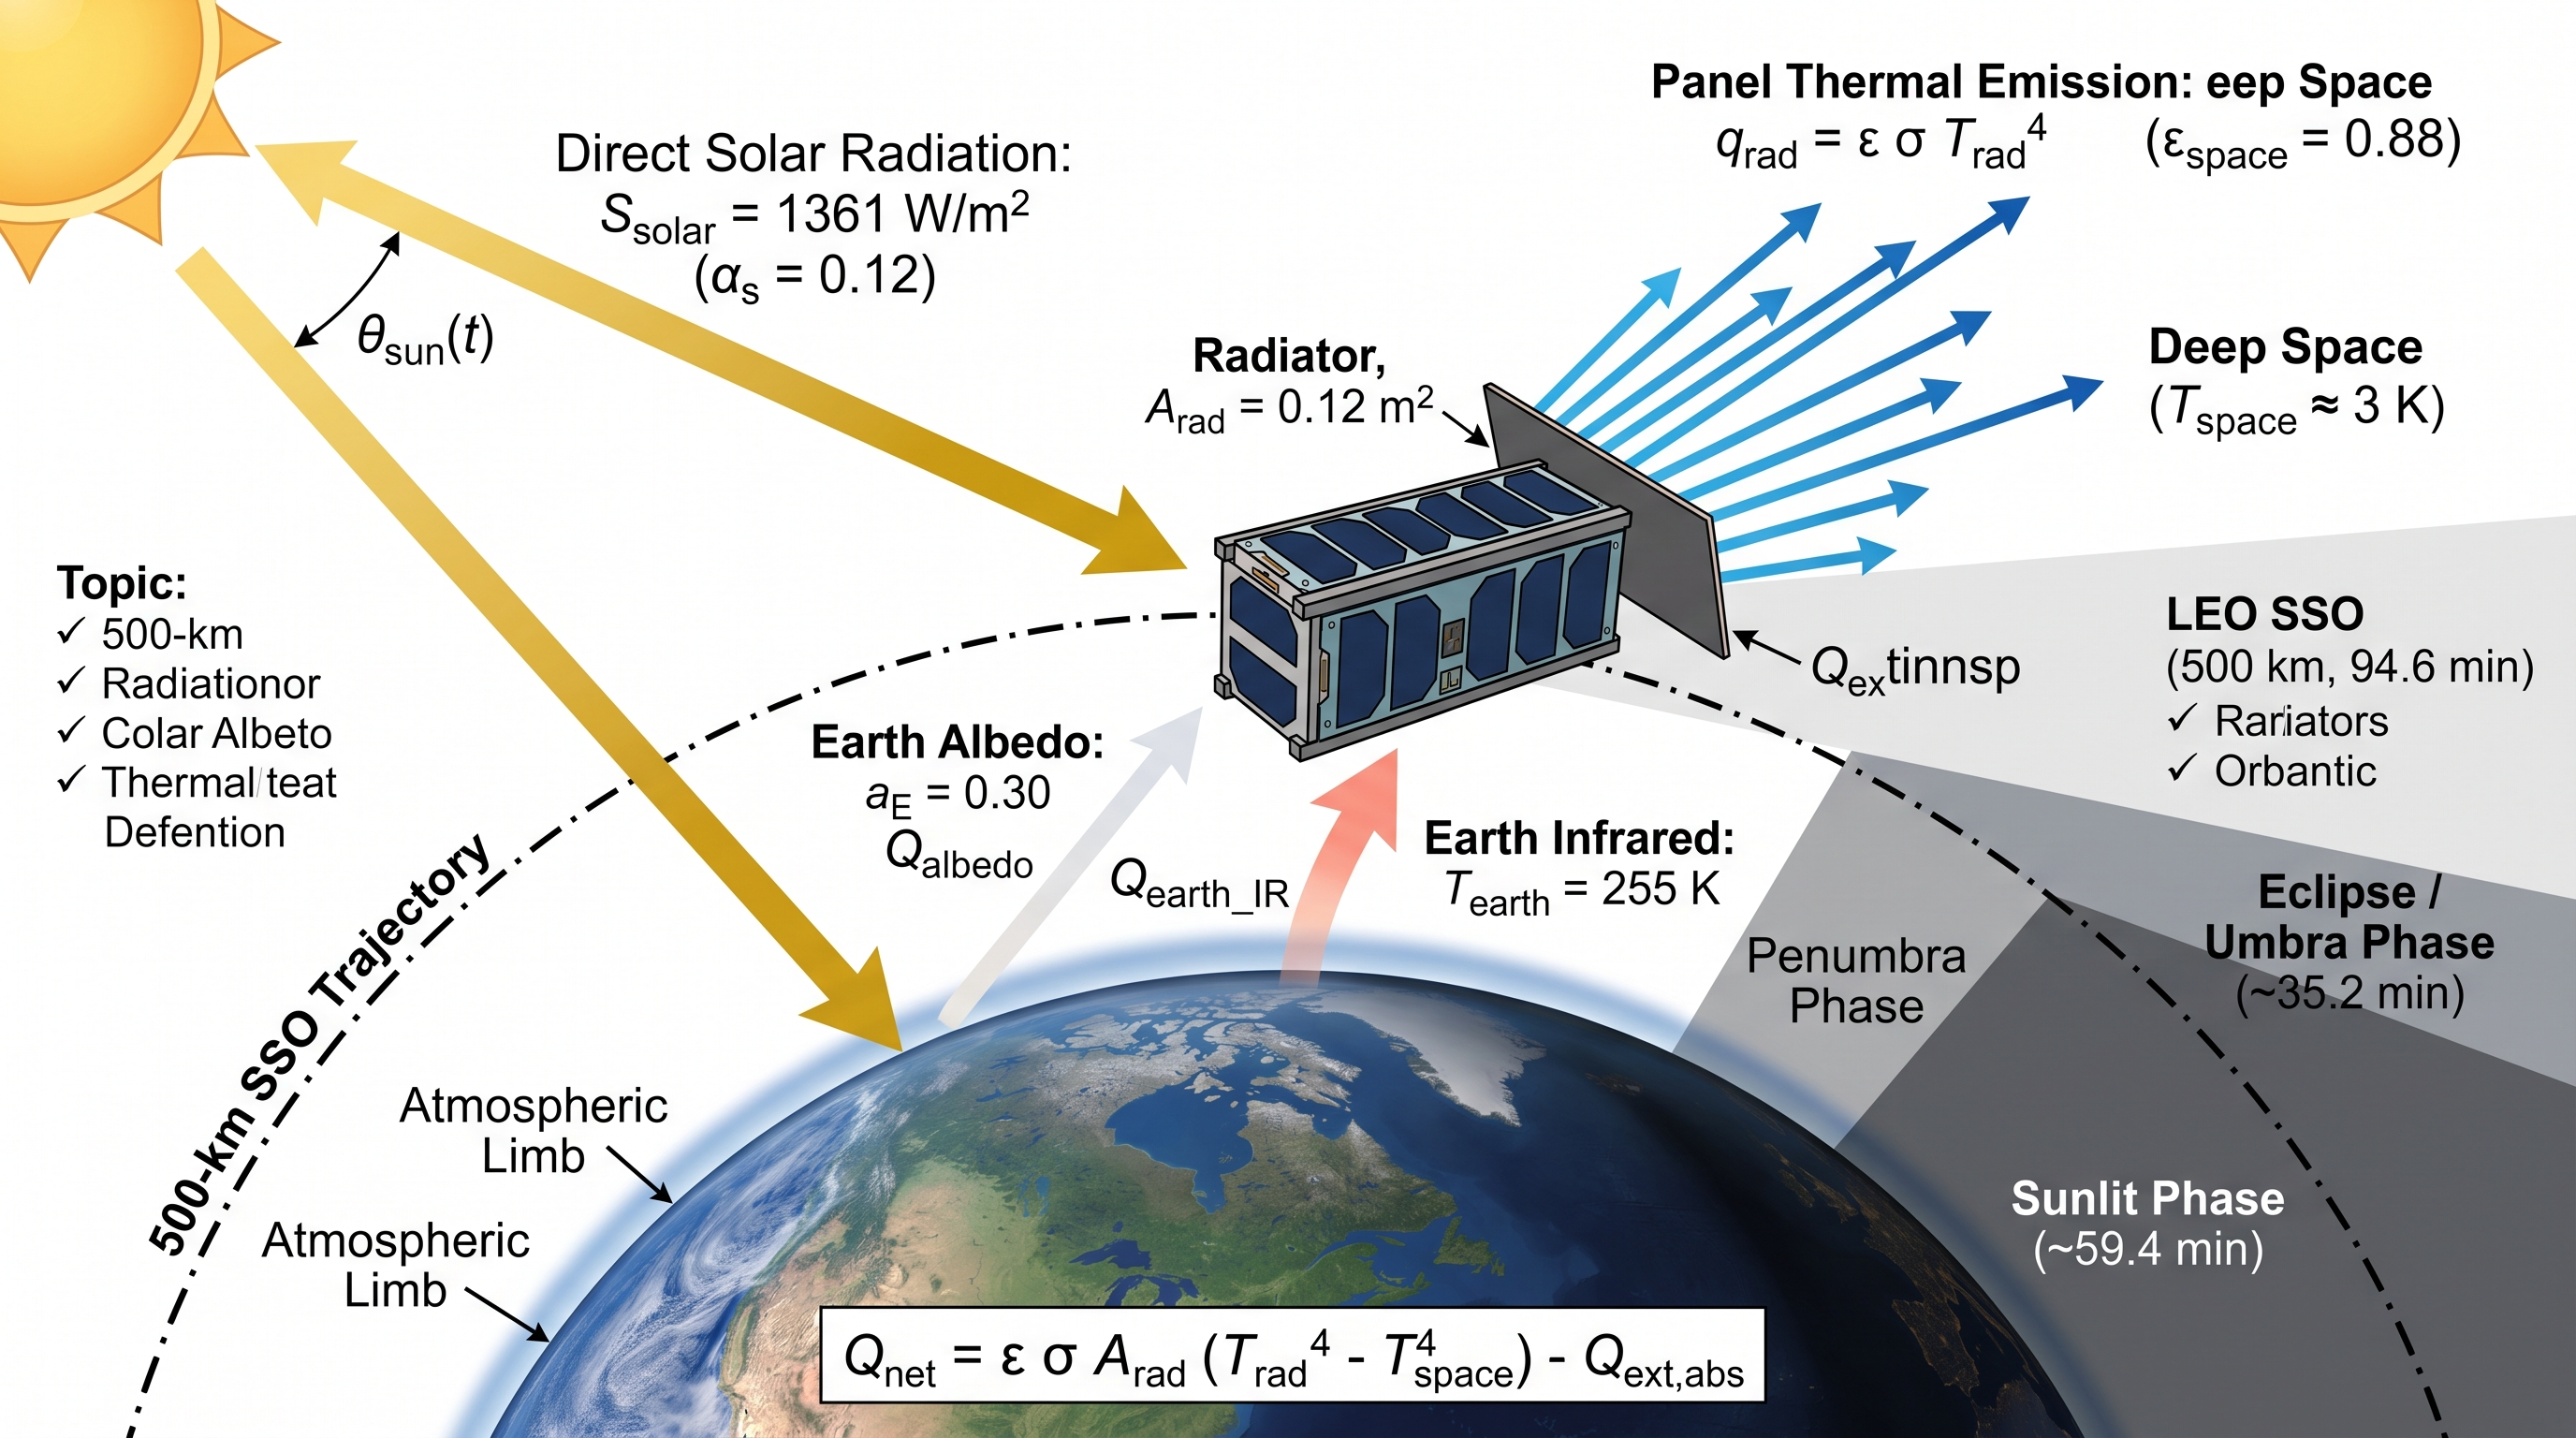
\includegraphics[width=0.98\columnwidth]{figuras/Gemini_Generated_Image_Figura01.jpg}
\caption{Synthetic 500~km circular LEO orbital geometry (Sun-Synchronous Orbit inclination $i \approx 97.4^\circ$, solar beta angle $\beta = 0^\circ$): direct solar flux, Earth albedo, terrestrial infrared emission, eclipse cone, and deep space radiator rejection. Conceptual rendering.}
\label{fig:geometria_orbital}
\end{figure}

\section{Orbital Environmental Physics and Heat Balance}
\label{sec:env}

\subsection{External Orbital Radiative Fluxes}
We consider a synthetic circular low Earth orbit thermal scenario at altitude $h = 500\text{ km}$ ($R = R_E + h = 6,871\text{ km}$), with analytical orbital period $T_{orb} = 5,668.14\text{ s}$ ($\approx 94.47\text{ min}$). Defining the orbital phase as $\varphi = \mathrm{mod}(t, T_{orb})/T_{orb}$, the illuminated orbital fraction is $\varphi_{sol} = 1 - \arcsin(R_E/R)/\pi$ under the conservative assumption of solar beta angle $\beta = 0^\circ$ (which maximizes eclipse duration and thermal shock amplitudes). With orbital solar noon at $\varphi_m = \varphi_{sol}/2$ and a smooth illumination operator $\mathbb{I}_{sun}(t) = [1 + e^{120(\varphi - \varphi_{sol})}]^{-1}$, the absorbed radiative fluxes on a radiator of area $A_{rad}$ (Fig.~\ref{fig:geometria_orbital}) are given by:
\begin{align}
\cos\theta_{ef}(t) &= \max\!\left[0,\ \cos\!\left(\tfrac{\pi(\varphi-\varphi_m)}{2\varphi_m}\right)\cos 30^\circ \cos 15^\circ\right], \\
Q_{sol}(t) &= \mathbb{I}_{sun}(t)\, S_{solar}\, \alpha_s A_{rad} \cos\theta_{ef}(t), \\
Q_{alb}(t) &= \mathbb{I}_{sun}(t)\, S_{solar}\, a_E\, \alpha_s A_{rad} F \cos\theta_{ef}(t), \\
Q_{IR}(t) &= \varepsilon \sigma A_{rad} F\, T_E^4(t), \\
T_E(t) &= 255 - 15\sin^2\!\left(\pi\tfrac{\varphi-\varphi_m}{\varphi_{sol}}\right),
\end{align}
where $S_{solar} = 1,361\text{ W/m}^2$ is the solar constant, $a_E = 0.30$ is the mean Earth albedo, $F = 0.42$ is the Earth-to-plate radiation view factor, $\alpha_s = 0.12$ is solar absorptivity, $\varepsilon = 0.88$ is infrared emissivity, and $\sigma = 5.67 \times 10^{-8}\text{ W/(m}^2\text{K}^4)$ is the Stefan-Boltzmann constant. Earth albedo is modeled proportionally to the illuminated visible fraction via $\cos\theta_{ef}$, a standard conservative approximation in spacecraft thermal engineering~\citep{ecss2008thermal, gilmore2002handbook}. The total external flux $Q_{ext}(t) = Q_{sol}(t) + Q_{alb}(t) + Q_{IR}(t)$ varies between 8.34~W (in eclipse) and 29.09~W (solar noon), with an orbital mean of 16.84~W.

\subsection{Passive Radiator Lumped Dynamics}
The thermal energy conservation equation for the radiator panel of mass $m_{rad}$ and specific heat $c_{p,rad}$ ($C_{rad} = m_{rad} c_{p,rad} = 1,299.2\text{ J/K}$) is governed by:
\begin{align}
C_{rad} \frac{dT_{rad}}{dt} = &\sum_{i=1}^{N} \frac{T_i - T_{rad}}{R_r} + Q_{ext}(t) \nonumber \\
&- \varepsilon \sigma A_{rad}\left(T_{rad}^4 - T_{space}^4\right),
\end{align}
where $R_r = 2.10\text{ K/W}$ represents the equivalent solid conductive thermal resistance between each die node and the radiator core.

\begin{figure}
\centering
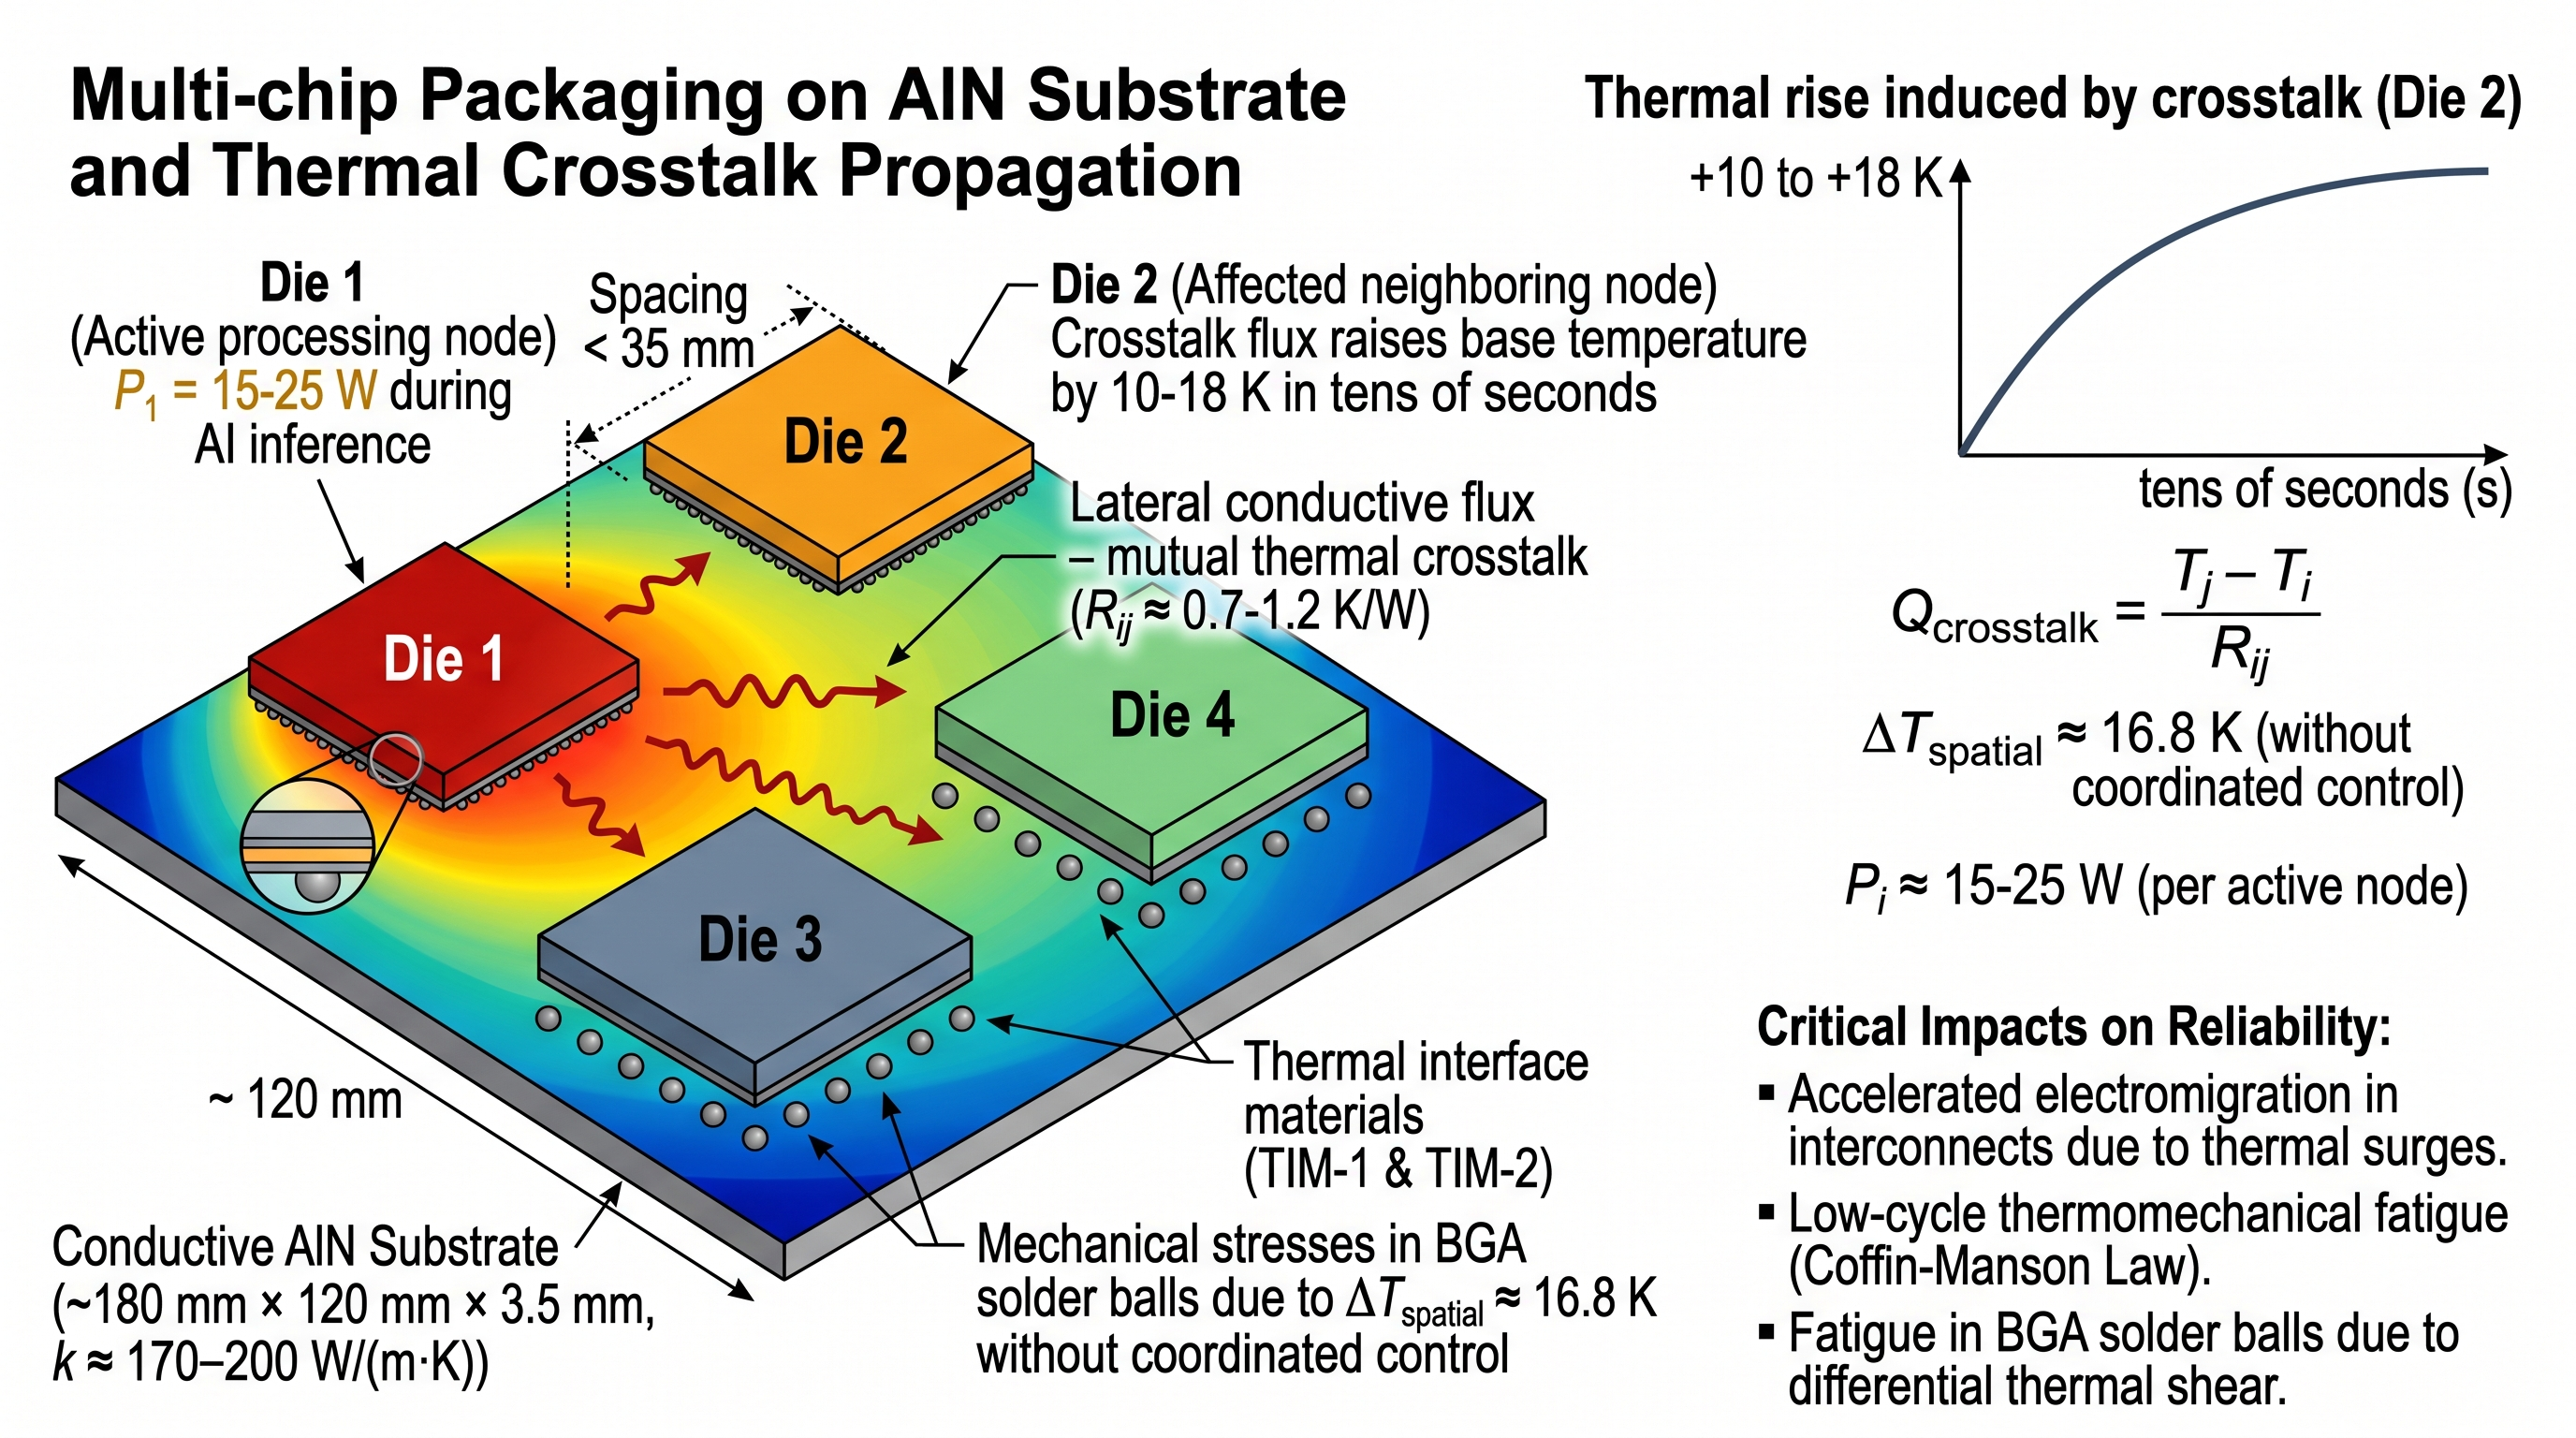
\includegraphics[width=0.98\columnwidth]{figuras/Gemini_Generated_Image_Figura03.jpg}
\caption{Solid conductive coupling and lateral thermal crosstalk in a multi-die carrier: heat dissipation in one node elevates base temperatures of adjacent dies and induces thermomechanical stress in BGA joints. Conceptual rendering.}
\label{fig:diafonia_3d}
\end{figure}

\section{State-Space Electrothermal Modeling}
\label{sec:model}

\subsection{Silicon Power Dissipation and Leakage Feedback}
Each silicon die (Fig.~\ref{fig:diafonia_3d}) dissipates electrical power partitioned into dynamic switching and subthreshold leakage components:
\begin{align}
V_i &= \mathrm{clip}\!\left(V_{min} + \beta_v (f_i - f_{min}),\, V_{min},\, V_{max}\right), \\
P_{dyn,i} &= \alpha_i C_{eff} V_i^2 f_i, \\
P_{leak,i} &= P_{ref} \left(\tfrac{V_i}{V_0}\right)^{1.5} \left(\tfrac{T_i}{T_0}\right)^2 \exp\!\left[\tfrac{E_a}{k_B}\left(\tfrac{1}{T_0} - \tfrac{1}{T_i}\right)\right],
\end{align}
where total power is $P_i = P_{dyn,i} + P_{leak,i}$, with $\alpha_i$ denoting active workload factor, $C_{eff} = 24.5\text{ nF}$ the effective switching capacitance, and $\beta_v = (V_{max}-V_{min})/(f_{max}-f_{min})$. Leakage power $P_{leak,i}$ exhibits a quadratic-exponential dependence on absolute junction temperature $T_i$, introducing non-linear positive electrothermal feedback ($\partial P_{leak}/\partial T_i > 0$) and a risk of thermal runaway in the absence of active intervention. Nominal parameters reflect commercial 16/12~nm FinFET embedded AI accelerators (Table~\ref{tab:params}). The subthreshold model is physically validated up to 125~$^\circ$C; operations above this ceiling are tagged as unphysical extrapolations ($^\dagger$).

\subsection{Compact Thermal Network ($5\times5$ CTM)}
The planar thermal coupling across an array of $N=4$ dies mounted on a shared AlN substrate is modeled by a lumped-parameter compact thermal network:
\begin{equation}
c_i \frac{dT_i}{dt} = P_i(t) - \sum_{j \ne i} \frac{T_i - T_j}{R_{ij}} - \frac{T_i - T_{rad}}{R_r},
\end{equation}
where $c_i = 18.5\text{ J/K}$ is the die thermal capacitance. In compact matrix notation:
\begin{equation}
\mathbf{C}\dot{\mathbf{T}} = \mathbf{P} - \left(\mathbf{G}_{crosstalk} + \mathbf{G}_{rad}\right)\mathbf{T} + \mathbf{G}_{rad} T_{rad}\mathbf{1}_N,
\end{equation}
where $\mathbf{C} = \mathrm{diag}(c_1, \dots, c_N)$, $\mathbf{G}_{rad} = R_r^{-1}\mathbf{I}_N$, and $\mathbf{G}_{crosstalk} \in \mathbb{R}^{N\times N}$ is the symmetric conductive Laplacian matrix:
\begin{equation}
[\mathbf{G}_{crosstalk}]_{ij} = \begin{cases} -1/R_{ij}, & i \ne j, \\ \sum_{k \ne i} 1/R_{ik}, & i = j. \end{cases}
\end{equation}
Modal decomposition of the die subsystem yields fast thermal time constants of 5.8, 7.5, 7.7, and 38.8~s, contrasting with the slow radiator time constant ($1.5\text{--}2.1\text{ ks}$). This pronounced two-time-scale separation provides thermodynamic justification for treating radiator temperature as a quasi-stationary state within the short-horizon predictive controller.

\begin{figure}
\centering
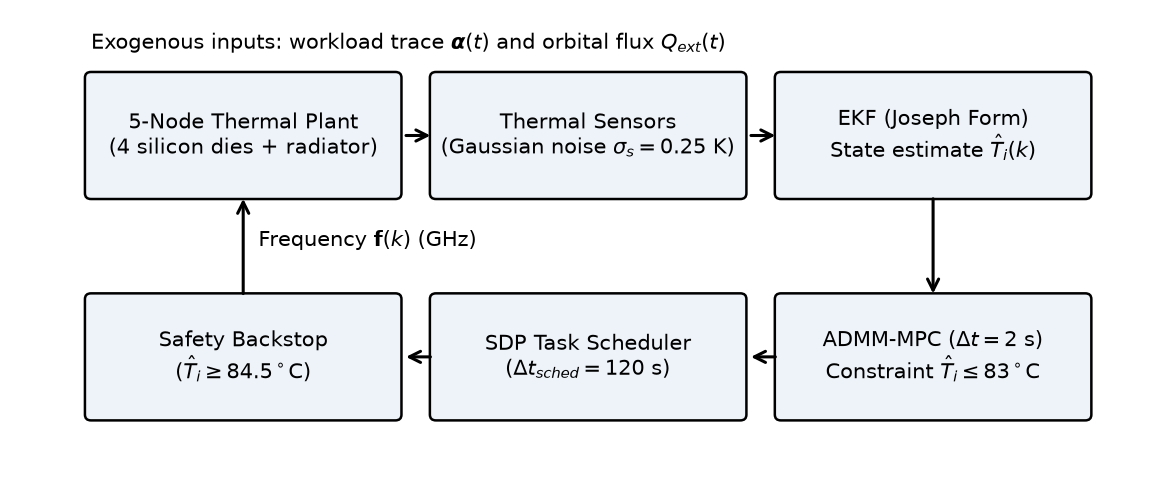
\includegraphics[width=0.98\columnwidth]{figuras/fig_arquitetura.png}
\caption{Closed-loop architecture of the TCAS-DVFS framework: non-linear $5\times5$ CTM plant, EKF state observer, orbital radiative power budgeter, topological SDP scheduler, and constrained discrete LTV MPC-DVFS controller.}
\label{fig:arquitetura}
\end{figure}

\section{Integrated TCAS-DVFS Control Architecture}
\label{sec:control}

The closed-loop control architecture (Fig.~\ref{fig:arquitetura}) operates on a multi-rate scheme: continuous physical plant integration and EKF state filtering operate at $\Delta t_{\text{plant}} = 0.5\text{ s}$, while model predictive control updates execute every $k_{sub} = 4$ steps ($\Delta t_{\text{MPC}} = 2.0\text{ s}$), and topological task allocation updates occur at $\Delta t_{sched} = 120\text{ s}$.

\subsection{State Estimation via Extended Kalman Filter}
The extended state vector $\mathbf{x} = [T_1, T_2, T_3, T_4, T_{rad}]^T \in \mathbb{R}^5$ is measured under zero-mean additive white Gaussian sensor noise: $\mathbf{y} = \mathbf{x} + \mathbf{v}$, $\mathbf{v} \sim \mathcal{N}(\mathbf{0}, \sigma_s^2\mathbf{I}_5)$, with standard deviation $\sigma_s = 0.25\text{ K}$~\citep{zhang2011tvlsi}. State propagation and covariance updates employ the stabilized Joseph form~\citep{simon2006optimal}:
\begin{align}
\hat{\mathbf{x}}^- &= \hat{\mathbf{x}}_{k-1} + \Delta t_{\text{plant}}\, \mathbf{f}(\hat{\mathbf{x}}_{k-1}, \mathbf{u}_{k-1}), \\
\boldsymbol{\Phi} &= \mathbf{I}_5 + \Delta t_{\text{plant}}\mathbf{F} + \tfrac{1}{2}(\Delta t_{\text{plant}}\mathbf{F})^2, \\
\mathbf{P}^- &= \boldsymbol{\Phi}\mathbf{P}\boldsymbol{\Phi}^T + \mathbf{Q}\Delta t_{\text{plant}}, \\
\mathbf{K} &= \mathbf{P}^-(\mathbf{P}^- + \mathbf{R})^{-1}, \quad \hat{\mathbf{x}} = \hat{\mathbf{x}}^- + \mathbf{K}(\mathbf{y} - \hat{\mathbf{x}}^-), \\
\mathbf{P} &= (\mathbf{I}_5-\mathbf{K})\mathbf{P}^-(\mathbf{I}_5-\mathbf{K})^T + \mathbf{K}\mathbf{R}\mathbf{K}^T,
\end{align}
where process noise covariance is $\mathbf{Q} = \mathrm{diag}(0.02\,\mathbf{I}_4,\, 0.05)$, measurement noise covariance is $\mathbf{R} = \sigma_s^2 \mathbf{I}_5$, initial error covariance is $\mathbf{P}_0 = \mathrm{diag}(\mathbf{I}_4,\, 2)$, and Jacobian $\mathbf{F} = \partial \mathbf{f}/\partial \mathbf{x}$ linearizes the Stefan-Boltzmann radiator flux ($g_{rad,lin} = 4\varepsilon\sigma A_{rad} \hat{T}_{rad}^3$). In closed-loop co-simulation, the observer achieves an average junction temperature tracking RMSE below $0.12\text{ K}$.

\subsection{Predictive Radiative Power Budget Surrogate}
Using onboard orbital ephemerides over the prediction horizon ($H_p = 30$ steps, 60.0~s), we compute a temperature-referenced radiative power-budget surrogate $P_{bud}(k)$ used as an MPC constraint surrogate to prevent the radiator from driving past steady-state equilibrium:
\begin{align}
P_{bud}(k) &= \max\Big\{15,\ \varepsilon\sigma A_{rad}\big[(T_{seg}+273.15)^4 \nonumber \\
&\quad - T_{space}^4\big] - \bar{Q}_{ext}(k)\Big\},
\end{align}
where $T_{seg} = 83^\circ\text{C}$ and $\bar{Q}_{ext}(k) = \frac{1}{H_p}\sum_{j=k}^{k+H_p-1}Q_{ext}(j)$ is the predicted moving-average environmental flux.

\subsection{Topological Task Scheduler (TCAS)}
At task allocation epochs ($\Delta t_{sched} = 120\text{ s}$), $M=4$ incoming neural inference workloads are assigned to the $N=4$ dies to minimize conductive crosstalk weighted by the steady-state impedance matrix $\mathbf{\Phi} = (\mathbf{G}_{crosstalk} + \mathbf{G}_{rad})^{-1}$:
\begin{equation}
\min_{\mathbf{X}} \sum_{i=1}^N \sum_{j=1}^N \Phi_{ij} P_i(\mathbf{X}) P_j(\mathbf{X}) + \mu \sum_{i=1}^N \left(T_i - \bar{T}\right)^2,
\end{equation}
subject to bijective task assignment constraints $\sum_{i=1}^N X_{pi} = 1$ and $\sum_{p=1}^M X_{pi} = 1$. Vectorizing the binary assignment decision matrix into $\mathbf{x} = \mathrm{vec}(\mathbf{X}) \in \{0, 1\}^{N^2}$ ($n = N^2 = 16$), the Shor semidefinite relaxation lifts the decision variable into the matrix cone:
\begin{equation}
\mathbf{Z} = \begin{bmatrix} 1 & \mathbf{x}^T \\ \mathbf{x} & \mathbf{X}_{lift} \end{bmatrix} \in \mathbb{S}_+^{N^2 + 1} = \mathbb{S}_+^{17}.
\end{equation}
Candidate discrete allocations are recovered via randomized hyperplane rounding~\citep{boyd2004convex}. For compact $N=4$ layouts, the exact permutation space contains $4! = 24$ configurations, permitting exhaustive ex-post validation of the discrete suboptimality gap; however, the SDP rounding procedure does not provide a certified dual lower bound in this implementation.

\subsection{Discrete Linear Time-Varying Model Predictive Control (LTV MPC-DVFS)}
To coordinate operating frequencies $\mathbf{f}(k) = [f_1, \dots, f_N]^T$ in real time, the control problem is formulated as a discrete Linear Time-Varying Model Predictive Controller executed at control interval $\Delta t_{\text{MPC}} = 2.0\text{ s}$ over a control horizon $H_c = 8$ steps (16.0~s) and prediction horizon $H_p = 30$ steps (60.0~s):
\begin{align}
\min_{\mathbf{f}, s} \sum_{j=1}^{H_c} \Big[ &w \|\mathbf{f}(k+j-1) - \mathbf{f}_{nom}(k+j-1)\|^2 \nonumber \\
&+ R_w \|\mathbf{D} \mathbf{f}(k+j-1)\|^2 \Big] \nonumber \\
&+ \rho \sum_{j=1}^{H_p} \|\tilde{\mathbf{T}}_{grad}(k+j)\|^2 + \lambda s^2,
\label{eq:mpc_cost}
\end{align}
\noindent subject to physical and operational constraints:
\begin{align}
f_{min} &\le f_i(k+j) \le f_{max}, \quad \forall i, j, \label{eq:mpc_f} \\
T_i(k+j|k) &\le T_{cap} + s, \quad s \ge 0, \label{eq:mpc_tcap} \\
\sum_{i=1}^N P_i(k+j|k) &\le P_{bud}(k+j), \quad \forall j, \label{eq:mpc_pbud}
\end{align}
where $w = 1.0$ penalizes deviation from nominal inference request $\mathbf{f}_{nom}$, $R_w = 0.2$ regularizes frequency change rate via the first-difference operator $\mathbf{D}$, $\rho = 0.02$ penalizes spatial temperature gradients relative to instantaneous spatial mean $\tilde{\mathbf{T}}_{grad} = \mathbf{T} - (\frac{1}{N}\mathbf{1}_N^T\mathbf{T})\mathbf{1}_N$, and $\lambda = 200.0$ penalizes the non-negative scalar thermal constraint slack variable $s \ge 0$ under nominal thermal cap $T_{cap} = 83.0^\circ\text{C}$.

The condensed quadratic program is solved using a warm-started ADMM-style splitting method~\citep{boyd2011admm, stellato2020osqp} with an over-relaxation parameter $\alpha = 1.6$, step size $\rho_{\mathrm{ADMM}} = 1.0$, regularization $\sigma = 10^{-6}$, and a fixed iteration cap of 60 iterations. Convergence tolerances ($\|Ax - z\|_\infty < 2\times 10^{-3}$) and primal/dual residuals are monitored at each control update. The state trajectory is warm-started using the shifted solution from the preceding control epoch. A fast proportional safety backstop operates at the plant rate ($\Delta t_{\text{plant}} = 0.5\text{ s}$), intervening if estimated temperatures exceed $84.5^\circ\text{C}$ to cap frequencies according to $f_i \le f_{nom,i} \max[0.15, (85.0 - T_i)/(85.0 - 75.0)]$.

\begin{table*}[t]
\caption{System Simulation, Electrothermal, and Orbital Parameters}
\label{tab:params}
\centering
\small
\begin{tabular*}{\textwidth}{@{\extracolsep{\fill}}p{0.24\textwidth}p{0.44\textwidth}p{0.28\textwidth}@{}}
\toprule
\textbf{Parameter Category} & \textbf{Symbol \& Description} & \textbf{Nominal Value \& Source} \\
\midrule
Conductive Resistances & $R_{12}=R_{34}$, $R_{13}=R_{24}$, $R_{14}=R_{23}$ & 1.45, 1.52, 3.20~K/W (MCM carrier model)~\citep{wang2025packaging} \\
Die-to-Radiator Resistance & $R_r$ (conductive thermal resistance per die node) & 2.10~K/W (Cold plate interface)~\citep{ecss2008thermal} \\
Thermal Capacitances & $c_i$ (silicon die node), $C_{rad}$ (radiator core $m\,c_p$) & 18.5~J/K (FinFET die), 1,299.2~J/K (1.45~kg Al) \\
Radiator Properties & $A_{rad}$ (area), $\varepsilon$ (emissivity), $\alpha_s$ (absorptivity) & 0.12~m$^2$, 0.88 (white paint), 0.12~\citep{pederson2024radiator} \\
Orbital Environment & $h$ (altitude), $T_{orb}$ (period), $F$ (view factor), $a_E$ (albedo) & 500~km, 5,668.14~s, 0.42, 0.30~\citep{gilmore2002handbook} \\
Electrical Operational & $V_{min}$--$V_{max}$, $f_{min}$--$f_{max}$ & 0.65--1.05~V, 0.30--1.30~GHz (16/12~nm FinFET) \\
Leakage Parameters & $C_{eff}$ (capacitance), $P_{ref}$ ($T_0=300\text{ K}$, $V_0=0.85\text{ V}$), $E_a$ & 24.5~nF, 0.80~W, 0.20~eV~\citep{kang2025power} \\
State Observer (EKF) & Sensor noise $\sigma_s$, Covariances $\mathbf{Q}$, $\mathbf{P}_0$, $\mathbf{R}$ & $\sigma_s=0.25\text{ K}$, $\mathbf{Q}=\mathrm{diag}(0.02, 0.02, 0.02, 0.02, 0.05)$, $\mathbf{R}=\sigma_s^2\mathbf{I}_5$ \\
MPC Formulation & $\Delta t_{\text{MPC}}$, $H_c$, $H_p$, $T_{cap}$, $T_{bar}$, Weights $w, R_w, \rho, \lambda$ & 2.0~s, 8 steps (16~s), 30 steps (60~s), 83.0~$^\circ$C, 84.5~$^\circ$C, $w=1.0, R_w=0.2, \rho=0.02, \lambda=200.0$ \\
Workload Benchmarks & Nominal inference throughputs ($\mathrm{FPS}_{nom}$) & SAR-YOLO (45), Cloud-Seg (60), Hyper-ViT (30), Telemetry (80) \\
\bottomrule
\end{tabular*}
\end{table*}

\section{Computational Simulation Methodology}
\label{sec:sim_method}

The multi-physics co-simulation platform was developed in Python 3.14 using NumPy, following verification and credibility principles for computational modeling and simulation~\citep{nasa2022handbook}. The numerical simulation contains 34,009 time samples and 34,008 integration intervals of $\Delta t_{\text{plant}} = 0.5\text{ s}$ integrated via a 2nd-order Runge-Kutta scheme (Heun / RK2), spanning 17,004.0~s, compared with an analytical three-orbit duration of approximately 17,004.43~s ($3 \times 5,668.14\text{ s}$). A formal temporal convergence study across $\Delta t_{\text{plant}} \in \{1.0, 0.5, 0.25, 0.125\}\text{ s}$ (with invariant control step $\Delta t_{\text{MPC}} = 2.0\text{ s}$) confirmed monotonic convergence: the nominal discretization ($\Delta t = 0.5\text{ s}$) incurs an absolute deviation of only $0.155\text{ K}$ in peak junction temperature ($T_{\max} = 83.21^\circ\text{C}$ vs. $83.06^\circ\text{C}$ at $\Delta t = 0.125\text{ s}$), a peak spatial gradient difference under $0.024\text{ K}$, and a relative total energy variance of $0.23\%$, remaining well below the sensor measurement noise floor ($\sigma_s = 0.25\text{ K}$).

\textbf{Benchmarking Protocol:}
To ensure strict methodological parity, all benchmarked governors evaluate:
\begin{enumerate}[(i)]
\item identical initial states $\mathbf{x}_0$ ($T_{i,0} = 310\text{ K}$, $T_{rad,0} = 270\text{ K}$);
\item identical synthetic inference workload request traces $\mathbf{f}_{nom}(t)$ and activity factors $\boldsymbol{\alpha}(t)$;
\item identical modeled orbital environmental radiative forcing $Q_{ext}(t)$;
\item identical stochastic sensor noise realizations for any given seed;
\item identical thermal plant model and integration steps.
\end{enumerate}

\textbf{Performance and Energy Proxies:}
Aggregate inference throughput is evaluated via the performance proxy:
\begin{equation}
\mathrm{FPS} = \frac{1}{N_{steps}}\sum_{t} \sum_{i=1}^N \frac{f_i(t)}{f_{max}}\,\mathrm{FPS}_{nom,i},
\end{equation}
and aggregate energy efficiency is quantified by the throughput-normalized energy-delay product proxy:
\begin{equation}
E_{t_{\mathrm{frame}}} = E \cdot \frac{1}{\mathrm{FPS}} \quad [\mathrm{kJ}\cdot\mathrm{s/frame}],
\end{equation}
where $E = \Delta t_{\text{plant}} \sum_t \sum_i P_i(t)$. Instantaneous inter-die spatial gradient is computed as $\Delta T_{esp}(t) = \max_i T_i(t) - \min_i T_i(t)$.

\textbf{Benchmarked Control Policies:}
\begin{enumerate}
\item \textit{Linux Ondemand:} standard reactive governor without thermal protection.
\item \textit{Ondemand + trip 95/85:} ondemand governor with emergency trip hysteresis at 95~$^\circ$C.
\item \textit{Thermal Throttling 85/75:} binary frequency drop to $f_{min}$ upon reaching 85~$^\circ$C with recovery at 75~$^\circ$C.
\item \textit{Thermal Throttling 83/73:} conservative baseline matched to the 83~$^\circ$C design margin.
\item \textit{Space-PID:} decentralized per-die PID controllers with gains selected from a predefined 27-point grid by minimizing an ITAE-based objective augmented with a thermal-violation penalty over the initial tuning interval ($K_p=-0.07$, $K_i=-0.002$, $K_d=-0.04$) set to regulate at 80~$^\circ$C.
\item \textit{Power Cap 65 W:} static global power budgeting enforced by the EPS.
\item \textit{TCA-DVFS (simple):} uncoordinated Laplacian rule with thermal barrier and radiative budget, excluding MPC and SDP.
\item \textbf{TCAS-DVFS (proposed):} full multi-rate architecture integrating EKF, topological SDP task allocation, and warm-started ADMM-based discrete LTV MPC-DVFS.
\end{enumerate}

All simulation source code, experimental pipelines, nominal configuration manifests (\texttt{configs/nominal.json}), convergence verification suites, ASTM E1049-85 validation test harnesses, and computational reproducibility metadata (\texttt{results/metadata.json}) are organized under an open-source MIT repository structure at \url{https://github.com/dafnhe-thor-barros/TCAS-DVFS}.

\section{Results and Discussion}
\label{sec:results}

\subsection{Global Performance Comparison}

\begin{table*}[t]
\caption{Consolidated Results in 3-Orbit LEO Co-Simulation (500~km SSO, 34,009 Steps, $\Delta t = 0.5$~s, Seed 0)}
\label{tab:results_completo}
\centering
\footnotesize
\setlength{\tabcolsep}{3pt}
\begin{tabular*}{\textwidth}{@{\extracolsep{\fill}}lcccccccc@{}}
\toprule
\textbf{Strategy} & \textbf{$T_{\text{mean}}$ ($^\circ$C)} & \textbf{$T_{\max}$ ($^\circ$C)} & \textbf{$\Delta T_{\text{peak}}$ (K)} & \textbf{$\Delta T_{\text{mean}}$ (K)} & \textbf{$t_{>85}$ (s)} & \textbf{FPS} & \textbf{$E_{t_{\mathrm{fr}}}$ (kJ$\cdot$s/fr)} & \textbf{Energy (kJ)} \\
\midrule
Linux Ondemand & 350.17$^\dagger$ & 412.30$^\dagger$ & 12.87 & 8.64 & 16,038.0 & 181.21$^\dagger$ & 28.38 & 5,143.3$^\dagger$ \\
Ondemand + trip 95/85 & 87.96 & 95.95 & 9.28 & 3.93 & 16,037.5 & 117.27 & 8.63 & 1,011.5 \\
Throttling 85/75 & 78.08 & 86.06 & 9.42 & 5.26 & 200.5 & 119.58 & 7.57 & 905.6 \\
Throttling 83/73 & 76.17 & 83.78 & 9.46 & 5.24 & 0.0 & 118.75 & 7.46 & 885.4 \\
Space-PID & 79.73 & 85.56 & 4.88 & 0.62 & 14.0 & 123.24 & 7.47 & 920.5 \\
Power Cap (65~W) & 93.95 & 109.31 & 5.82 & 3.66 & 14,983.5 & 126.49 & 8.55 & 1,081.3 \\
TCA-DVFS (simple) & 80.53 & 83.74 & 1.58 & 0.45 & 0.0 & 116.16 & 8.03 & 932.4 \\
\midrule[\heavyrulewidth]
\textbf{TCAS-DVFS (Proposed)} & \textbf{80.28} & \textbf{83.27} & \textbf{2.11} & \textbf{0.80} & \textbf{0.0} & \textbf{124.38} & \textbf{7.48} & \textbf{930.0} \\
\bottomrule
\end{tabular*}
\par\vspace{2pt}\footnotesize
$^\dagger$ Regimes beyond model validity ceiling ($>125^\circ$C). Linux Ondemand experiences thermal runaway under positive subthreshold leakage feedback, reaching 412.30~$^\circ$C and dissipating an unphysical average of 302.5~W. This regime represents numerical extrapolation failure and is strictly excluded from quantitative reliability and performance inferences. Overshoot to 86.06~$^\circ$C in Throttling 85/75 stems from sampling latency and sensor noise.
\end{table*}

Table~\ref{tab:results_completo} presents the consolidated comparative results across 3 full orbits. \textbf{TCAS-DVFS} successfully maintained junction temperatures strictly below the 85~$^\circ$C flight envelope, registering a peak of $83.27^\circ\text{C}$ and \textbf{zero observed seconds of thermal violation} ($0.00\%$). In contrast, standard Thermal Throttling 85/75 accumulated 200.5~s of overheating due to hysteresis latency, and Space-PID breached the limit for 14.0~s during the post-eclipse thermal shock.

In terms of processing throughput, TCAS-DVFS delivered 124.38~FPS, outperforming Throttling 85/75 (+4.0\%) and conservative Throttling 83/73 (+4.7\%), while matching energy-delay efficiency ($7.477\text{ kJ}\cdot\text{s/frame}$ versus $7.456\text{ kJ}\cdot\text{s/frame}$). Relative to simple uncoordinated TCA-DVFS (116.16~FPS, $8.027\text{ kJ}\cdot\text{s/frame}$), the constrained MPC controller delivered a +7.1\% throughput boost and a 6.8\% reduction in $E_{t_{\mathrm{frame}}}$, demonstrating the practical efficacy of active multivariable coordination.

\begin{table}[t]
\caption{Statistical Dispersions across 10 Stochastic Sensor Noise Seeds (Seeds 0 to 9)}
\label{tab:sementes}
\centering
\footnotesize
\setlength{\tabcolsep}{1.5pt}
\begin{tabular*}{\columnwidth}{@{\extracolsep{\fill}}lccc@{}}
\toprule
\textbf{Metric} & \textbf{Throttling 85/75} & \textbf{Space-PID} & \textbf{TCAS-DVFS} \\
\midrule
$T_{\max}$ ($^\circ$C) & $85.89 \pm 0.15$ & $85.54 \pm 0.04$ & $\mathbf{83.25 \pm 0.03}$ \\
$t_{>85}$ (s) & $213.5 \pm 15.7$ & $14.6 \pm 0.7$ & $\mathbf{0.0 \pm 0.0}$ \\
$\Delta T_{\text{peak}}$ (K) & $9.48 \pm 0.09$ & $4.86 \pm 0.02$ & $\mathbf{2.10 \pm 0.02}$ \\
$\Delta T_{\text{mean}}$ (K) & $5.26 \pm 0.13$ & $0.617 \pm 0.001$ & $\mathbf{0.795 \pm 0.001}$ \\
FPS & $119.70 \pm 0.35$ & $123.24 \pm 0.00$ & $\mathbf{124.38 \pm 0.00}$ \\
$E_{t_{\mathrm{frame}}}$ (kJ$\cdot$s/frame) & $7.566 \pm 0.024$ & $7.469 \pm 0.000$ & $\mathbf{7.477 \pm 0.000}$ \\
Energy (kJ) & $905.6 \pm 0.3$ & $920.46 \pm 0.01$ & $\mathbf{929.95 \pm 0.01}$ \\
\bottomrule
\end{tabular*}
\end{table}

Table~\ref{tab:sementes} details performance across 10 independent stochastic noise seeds. EKF filtering maintains maximum temperature dispersion to within $\pm 0.03\text{ K}$ in TCAS-DVFS, compared to $\pm 0.15\text{ K}$ for Throttling.

\subsection{Thermal Dynamics and Gradient Suppression}

\begin{figure*}
\centering
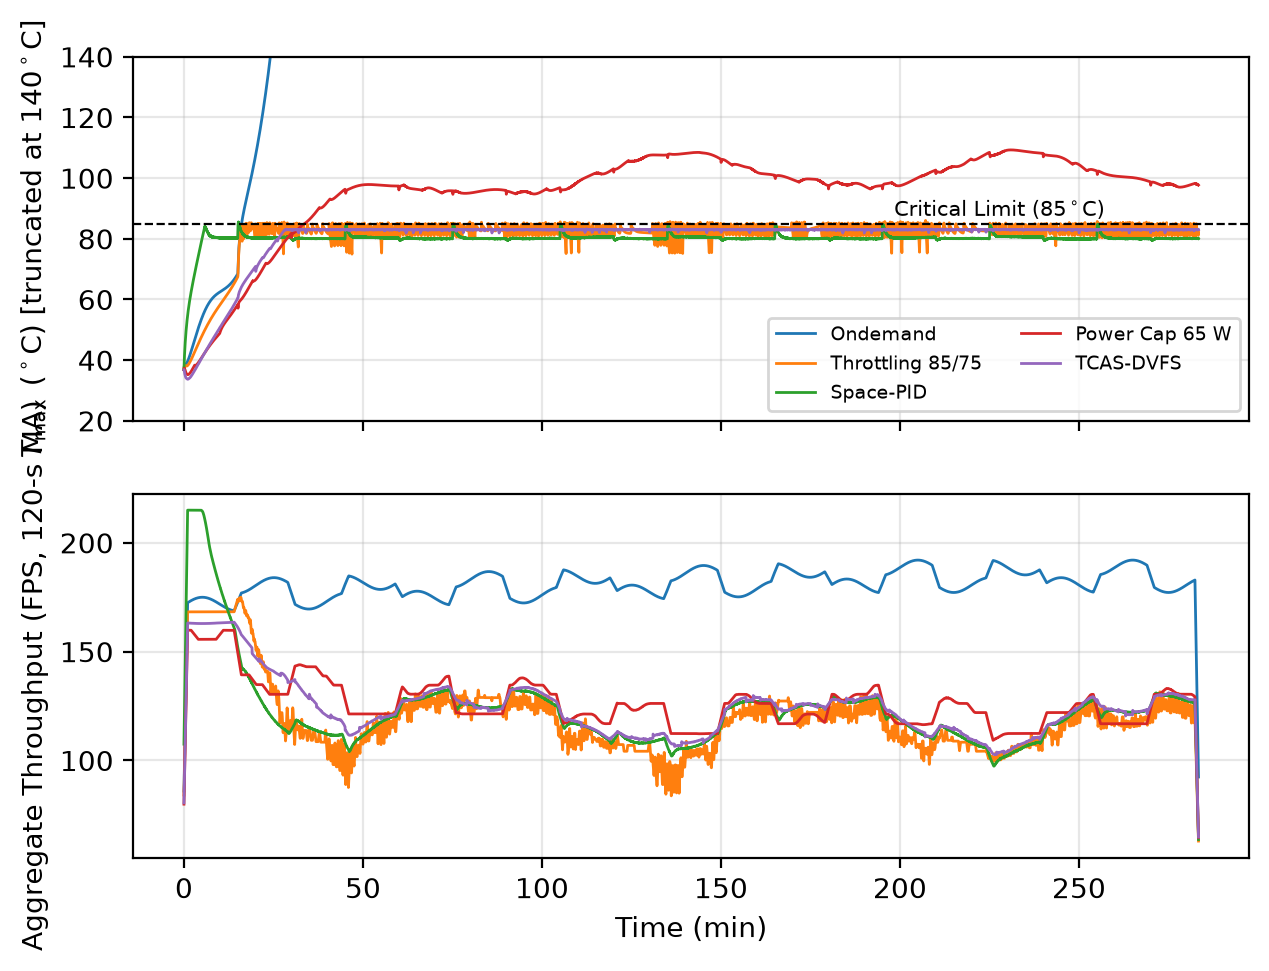
\includegraphics[width=0.88\textwidth]{figuras/fig_transiente.png}
\caption{Temporal co-simulation dynamics over 3 complete orbits (seed 0): (a) maximum silicon junction temperature ($T_{\max}$), demonstrating strict compliance of TCAS-DVFS below 85~$^\circ$C versus saw-tooth hysteresis in Throttling; (b) aggregate AI inference throughput smoothed with a 120~s moving average.}
\label{fig:transiente}
\end{figure*}

\begin{figure}
\centering
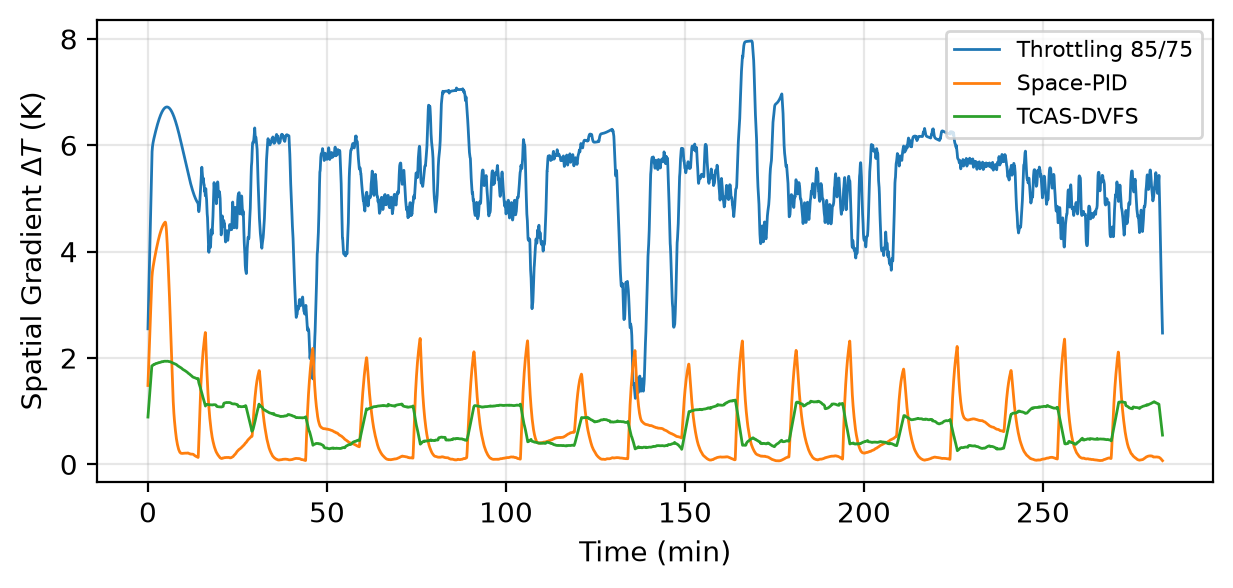
\includegraphics[width=0.98\columnwidth]{figuras/fig_gradiente.png}
\caption{Temporal evolution of inter-die spatial thermal gradient ($\Delta T_{esp}(t) = \max_i T_i - \min_i T_i$) with a 120~s moving average: active suppression of conductive crosstalk by TCAS-DVFS.}
\label{fig:gradiente}
\end{figure}

\begin{figure}
\centering
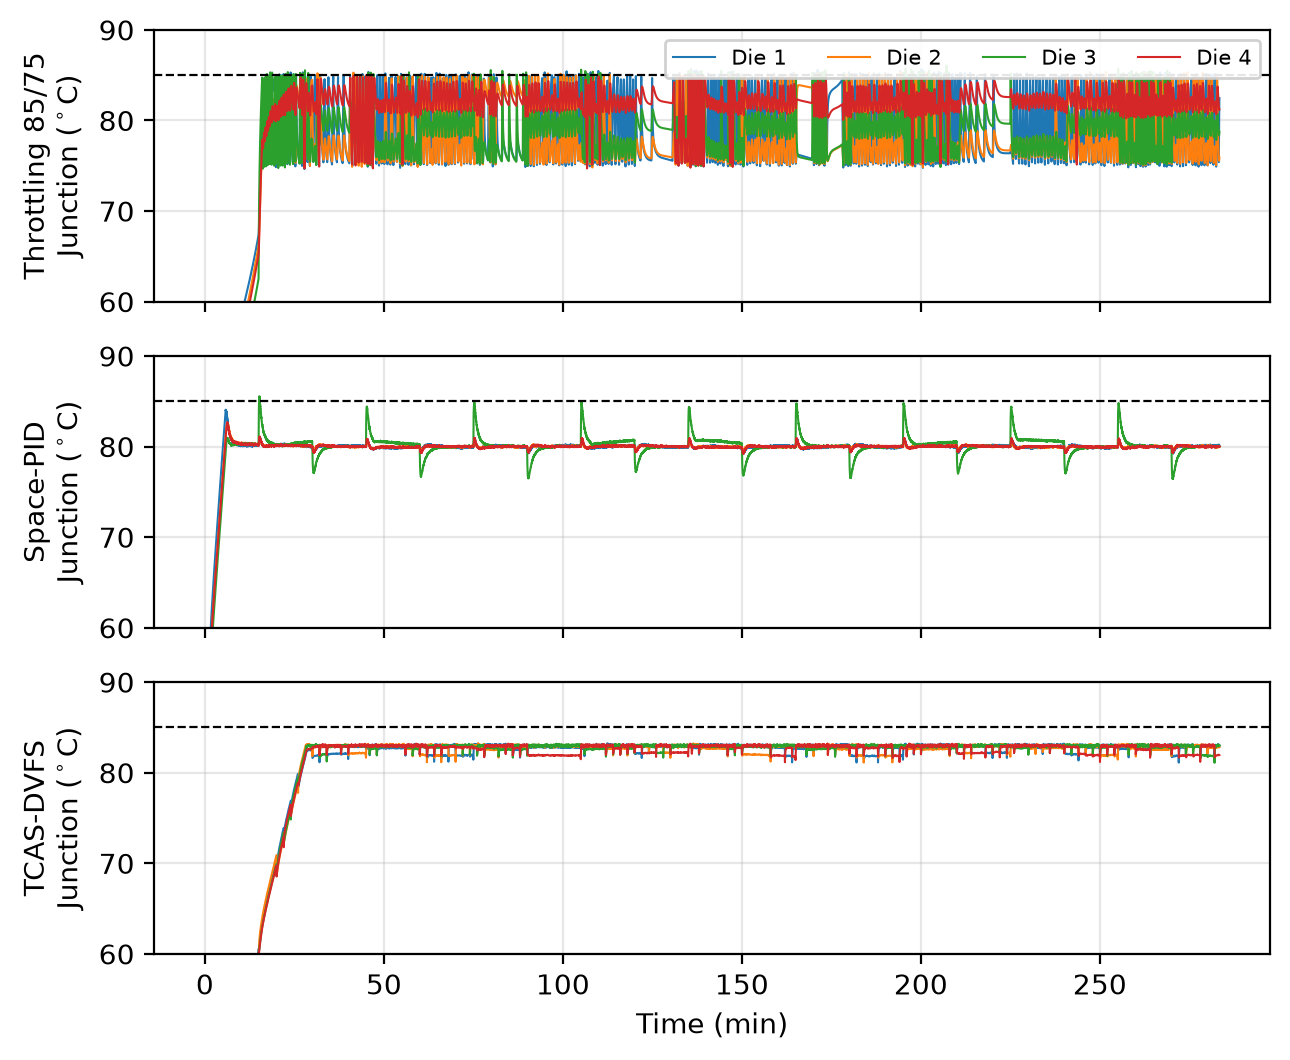
\includegraphics[width=0.98\columnwidth]{figuras/fig_trajetorias.png}
\caption{Individual junction temperature profiles for the 4 silicon dies (seed 0): homogeneous convergence under coordinated TCAS-DVFS versus spatial divergence under classical baselines.}
\label{fig:trajetorias}
\end{figure}

Figs.~\ref{fig:transiente}, \ref{fig:gradiente}, and \ref{fig:trajetorias} illustrate the orbital transient responses. While Throttling induces saw-tooth oscillations near 10~K and Space-PID exhibits gradient excursions during daylight transitions ($\Delta T_{\text{peak}} = 4.88\text{ K}$), TCAS-DVFS dampens mean gradients to $0.80\text{ K}$ and peak gradients to $2.11\text{ K}$ (a 77.6\% reduction relative to Throttling). Operating temperatures remained above 83~$^\circ$C for 57.7\% of the orbital period (9,818~s out of 17,004.5~s), confirming that the predictive controller deliberately tracks the upper thermal boundary to maximize compute throughput.

\subsection{Functional Ablation Study}
\label{sec:ablacao}

\begin{table*}[t]
\caption{Functional Ablation Study of TCAS-DVFS (3 Orbits, Seed 0)}
\label{tab:ablacao}
\centering
\small
\begin{tabular*}{\textwidth}{@{\extracolsep{\fill}}lcccccc@{}}
\toprule
\textbf{Variant} & $T_{\max}$ ($^\circ$C) & $\Delta T_{\text{peak}}$ (K) & $\Delta T_{\text{mean}}$ (K) & FPS & $E_{t_{\mathrm{frame}}}$ (kJ$\cdot$s/frame) & $t_{>85}$ (s) \\
\midrule
Full ($H_p=30$, 60.0~s) & 83.27 & 2.11 & 0.80 & 124.38 & 7.48 & 0.0 \\
Without SDP & 83.24 & 2.01 & 0.75 & 125.16 & 7.44 & 0.0 \\
Without MPC & 85.48 & 7.47 & 0.98 & 112.76 & 8.45 & 1,732.0 \\
$H_p = 10$ (20.0~s) & 83.27 & 2.10 & 0.80 & 124.38 & 7.48 & 0.0 \\
$H_p = 60$ (120.0~s) & 83.27 & 2.11 & 0.79 & 124.38 & 7.48 & 0.0 \\
Simple TCA & 83.74 & 1.58 & 0.45 & 116.16 & 8.03 & 0.0 \\
\bottomrule
\end{tabular*}
\end{table*}

The ablation results in Table~\ref{tab:ablacao}, re-evaluated across 3 full orbits for methodological consistency, isolate the architectural mechanisms:
\begin{itemize}
\item \textbf{Dominant observed contribution of MPC-DVFS in the tested configuration:} removing the MPC controller (\textit{Without MPC}) immediately leads to thermal threshold exceedance, accumulating 1,732.0~s above 85~$^\circ$C, a peak of $85.48^\circ\text{C}$, and a tripling of peak gradient to $7.47\text{ K}$. Dynamic lookahead within the MPC is the primary driver of proactive containment.
\item \textbf{Limited observed benefit of SDP scheduling for the tested $N=4$ configuration:} the \textit{Without SDP} variant (static task assignment) achieves performance essentially identical to the full framework ($83.24^\circ\text{C}$, $125.16\text{ FPS}$, $7.435\text{ kJ}\cdot\text{s/frame}$). The SDP allocator performed 262 task migrations and matched the ex-post optimal discrete permutation in 49 of 142 calls (34.5\%). In small symmetric configurations ($N=4$), conductive cross-coupling is spatially uniform, rendering topological remapping largely ineffective. Whether topology-aware scheduling becomes beneficial for larger and less symmetric arrays remains an open question.
\item \textbf{No material difference observed at the reported precision for the tested horizons:} varying prediction horizon $H_p \in \{10, 30, 60\}$ steps (corresponding to physical lookahead intervals of 20.0, 60.0, and 120.0~s under $\Delta t_{\text{MPC}} = 2.0\text{ s}$) produced identical performance metrics ($124.38\text{ FPS}$, $7.477\text{ kJ}\cdot\text{s/frame}$). This enables adopting shorter horizons ($H_p=10$) to minimize onboard processor utilization.
\end{itemize}

\subsection{Parametric Sensitivity Analysis (Latin Hypercube Sampling, $n=30$)}
\label{sec:incerteza}
To rigorously assess sensitivity against manufacturing dispersions and environmental deviations, a 30-sample Latin Hypercube Sampling (LHS) campaign was conducted (3 full orbits per sample, evaluating 1,020,270 integration steps) with simultaneous continuous uniform perturbations of $\pm20\%$ across $R_{ij}$, $R_r$, $c_i$, and $C_{rad}$ forming a parametric stress-test envelope.

No thermal-threshold violations were observed in the 30 sampled uncertainty realizations ($0/30$ samples $> 85^\circ\text{C}$). By the exact Clopper-Pearson method, the two-sided 95\% confidence upper bound for violation probability is \textbf{11.57\%}. Thus, while the campaign demonstrates robust containment within the sampled envelope, it does not establish a zero underlying violation probability (in contrast to Throttling 85/75, which violated thresholds in 100\% of samples with a mean violation time of $234.8\text{ s}$).

In paired comparisons under identical physical parameters:
\begin{enumerate}[(i)]
\item \textit{Versus Throttling 83/73}: TCAS-DVFS reduced peak temperatures by $0.63\text{ K}$ (95\% CI: $[-0.75, -0.50]\text{ K}$) and improved inference throughput by $+5.26\%$ (95\% CI: $[+4.60\%, +5.91\%]$). The EDP delta was $-0.36\%$ (95\% CI: $[-0.89\%, +0.18\%]$); because this interval crosses zero, \textbf{we make no claim of strict EDP superiority under uncertainty against Throttling 83/73}.
\item \textit{Versus Throttling 85/75}: TCAS-DVFS reduced peak temperature by $2.66\text{ K}$, raised throughput by $+4.38\%$, and achieved an EDP reduction of $-1.77\%$ (95\% CI: $[-2.31\%, -1.23\%]$).
\end{enumerate}

Within the sampled four-parameter uncertainty space, $R_r$ exhibited the strongest monotonic association with $T_{\max}$, with Spearman rank correlation $\rho = +0.994$, followed by die heat capacity $c_{\text{die}}$ ($\rho = -0.350$), radiator capacitance $C_{rad}$ ($\rho = -0.220$), and inter-die crosstalk resistance $R_{ij}$ ($\rho = -0.147$).

\section{Indicative Reliability and Physical Degradation Assessment}
\label{sec:reliability}

All reliability projections utilize thermal histories after discarding the initial 2-hour transient warm-up phase, and are presented strictly as indicative comparative proxies.

\subsection{Electromigration (Black's Equation Damage Proxy)}
A relative Black-equation damage-rate proxy was computed from the simulated electrical-power and junction-temperature histories~\citep{black1969electromigration}:
\begin{equation}
\mathrm{MTTF}_{EM} \propto J^{-n} \exp\!\left(\frac{E_{a,EM}}{k_B T_j}\right),
\end{equation}
where $n = 1.8$, $E_{a,EM} = 0.70\text{ eV}$, and current density is approximated by the normalized electrical current $J \propto P/V$. Time-integral accumulation over 3 orbits yielded relative MTTF proxy ratios ($\mathrm{MTTF}_{prop}/\mathrm{MTTF}_{ref}$) of \textbf{0.96} (aggregate dies) and 1.52 (worst die) versus Throttling 85/75; and \textbf{0.81} and 1.33 versus Throttling 83/73. Because TCAS-DVFS draws $+7.6\%$ and $+9.9\%$ higher average current due to sustained workload execution, we formally conclude that \textbf{the framework provides no net electromigration life extension}.

\subsection{Thermomechanical Solder Fatigue (Coffin-Manson Cyclic Severity)}
Cumulative low-cycle thermal cycling severity in SAC305 solder interconnects is estimated using the Coffin-Manson relation~\citep{manson1966fatigue}:
\begin{equation}
N_f = B\,(\Delta T_{cycle})^{-q}, \quad q = 2.1.
\end{equation}
Applying a three-point rainflow algorithm formally validated against the standard test sequences of ASTM E1049-85 (Section 5.4.4) and synthetic benchmarks to confirm exact peak-to-peak range counting ($\Delta T = T_{\text{peak}} - T_{\text{valley}}$), the maximum cyclic thermal excursion after transient warm-up dropped from $11.2\text{ K}$ (Throttling) to $2.12\text{ K}$ (TCAS-DVFS).

\begin{table}[t]
\caption{Rainflow Cycle Counting and Relative Fatigue Damage Severity Ratios ($q=2.1$, Aggregate Dies)}
\label{tab:cm}
\centering
\footnotesize
\setlength{\tabcolsep}{2pt}
\begin{tabular*}{\columnwidth}{@{\extracolsep{\fill}}cccc@{}}
\toprule
\textbf{Threshold} & \textbf{Cycles} & \textbf{Cycles} & \textbf{Damage Ratio} \\
\textbf{($\Delta T$)} & \textbf{Throttling} & \textbf{TCAS-DVFS} & \textbf{($D_{\text{thr}}/D_{\text{prop}}$)} \\
\midrule
0.25~K & 741 & 377 & 190.8 \\
1.00~K & 724 & 104 & 251.8 \\
2.00~K & 612 & 20 & 1,068.1 \\
\bottomrule
\end{tabular*}
\end{table}

\begin{figure}
\centering
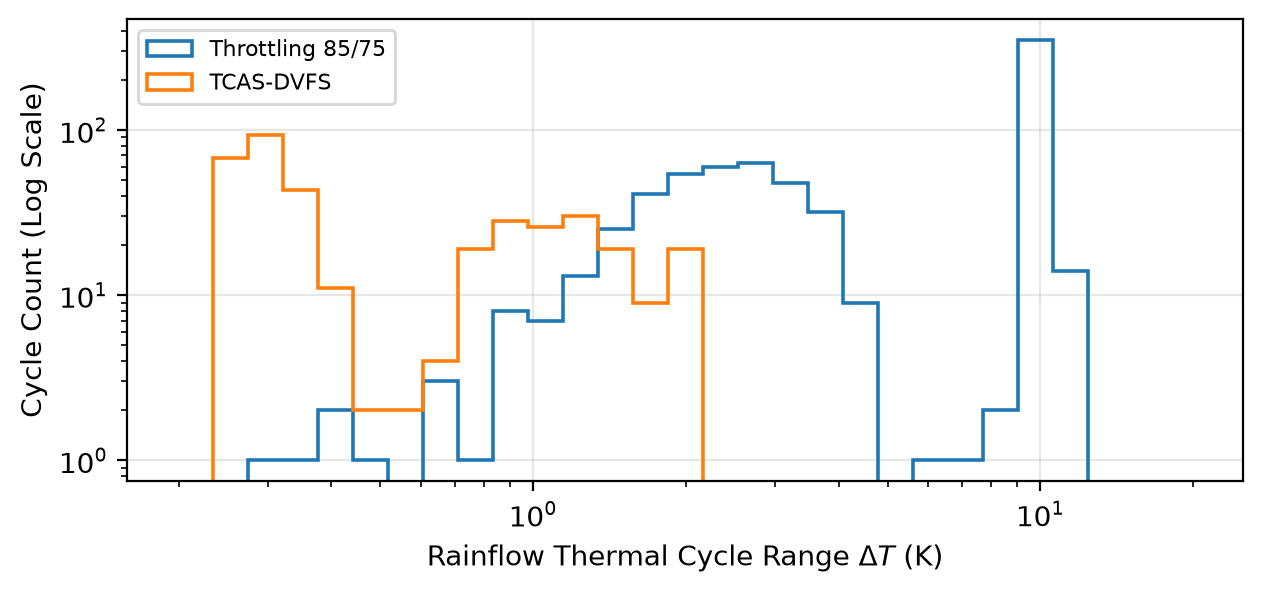
\includegraphics[width=0.98\columnwidth]{figuras/fig_confiabilidade.png}
\caption{Rainflow thermal cycle range spectrum ($\Delta T$, 0.25~K threshold after warm-up): TCAS-DVFS suppresses nearly all damaging cycles ($\Delta T > 2\text{ K}$).}
\label{fig:confiabilidade}
\end{figure}

As shown in Table~\ref{tab:cm} and Fig.~\ref{fig:confiabilidade}, eliminating large thermal excursions ($\Delta T > 2\text{ K}$) noticeably slows theoretical cyclic fatigue accumulation. However, junction temperature serves strictly as an indicative proxy for thermal cycling amplitude severity, rather than viscoplastic shear strain in actual solder joints. Comprehensive finite-element thermomechanical analysis remains required for flight qualification.

\section{Related Work}
\label{sec:related}

Dynamic Thermal Management (DTM) in terrestrial multi-core architectures has been extensively investigated using tools such as HotSpot~\citep{skadron2004hotspot, brooks2001dtm}. 3D floorplanning~\citep{lin2021thermal}, distributed task migration~\citep{ge2010distributed}, and convex frequency optimization~\citep{murali2007convex} advanced thermal regulation under convective conditions. In the aerospace domain, autonomous execution was validated by \citet{sherwood2003ase}, while advanced packaging models were proposed by \citet{wang2025packaging}, and GPU orbital thermal behavior was characterized by \citet{yuan2025heat}. The closest prior work is by \citet{chen2026hotai}, which formulated thermal crosstalk scheduling. Table~\ref{tab:relacionados} positions our contribution relative to the state of the art.

\begin{table}[t]
\caption{Positioning against Closely Related Prior Work}
\label{tab:relacionados}
\centering
\footnotesize
\setlength{\tabcolsep}{1.5pt}
\begin{tabular*}{\columnwidth}{@{\extracolsep{\fill}}lcccc@{}}
\toprule
\textbf{Work} & \textbf{Sched.} & \textbf{Pred. DVFS} & \textbf{EKF} & \textbf{$T^4$ + Ecl.} \\
\midrule
\citet{murali2007convex} & No & Static & No & No \\
\citet{yuan2025heat} & No & No & No & Empirical \\
\citet{chen2026hotai} & Yes & No & No & No \\
\textbf{This Work} & \textbf{Yes} & \textbf{LTV MPC} & \textbf{Yes} & \textbf{Yes} \\
\bottomrule
\end{tabular*}
\end{table}

\section{Practical Implementation Considerations and Threats to Validity}
\label{sec:practice}

\subsection{Implementation Constraints}
Deploying TCAS-DVFS on spaceborne flight computers requires addressing real-time execution constraints:
\begin{enumerate}
\item \textbf{Execution Complexity:} Embedded execution time, memory footprint, and worst-case timing remain to be benchmarked on flight-representative hardware. The warm-started ADMM-style iteration operates with a fixed cap of 60 iterations and early exit monitoring to prevent execution overruns.
\item \textbf{Memory Footprint:} The complete EKF covariance matrices, discrete prediction models, and warm-start vectors require modest scratchpad memory fitting within typical rad-hard microcontrollers.
\end{enumerate}

\subsection{Threats to Validity}
As a model-based numerical investigation, several limitations must be explicitly recognized:
\begin{enumerate}
\item \textbf{Absence of Physical and Environmental Testing:} The findings rely entirely on numerical simulation of the stated lumped-parameter thermal network and have not been validated via Hardware-in-the-Loop (HIL) testbeds or Thermal Vacuum (TVAC) chamber testing.
\item \textbf{Lumped Modeling vs.\ Continuum Physics:} While the $5\times5$ CTM captures inter-die conductive coupling and bulk radiator dynamics, it does not resolve spatial micro-gradients across silicon dies, localized hot spots, or three-dimensional heat spreader diffusion.
\item \textbf{Throughput and Reliability Proxies:} Workload throughput is evaluated via a linear frequency proxy rather than cycle-accurate kernel profiling. Similarly, Black's equation and Coffin-Manson models are indicative proxies based on temperature histories rather than direct measurements of current density or plastic strain.
\item \textbf{Omission of Space Radiation Effects:} The present study focuses strictly on electrothermal dynamics and does not model Single Event Effects (SEE) or Total Ionizing Dose (TID), which can affect DVFS stability and memory integrity in orbital environments.
\end{enumerate}

\section{Conclusions}
\label{sec:concl}
This paper presented TCAS-DVFS, a predictive control framework designed to mitigate spatial thermal crosstalk in high-density spaceborne AI clusters operating in deep orbital vacuum. The conclusions of this model-based numerical study are delineated into three levels:
\begin{enumerate}
\item \textbf{Demonstrated in the nominal model:} Integrated EKF state estimation, temperature-referenced radiative power budgeting, and discrete LTV MPC-DVFS produced zero observed thermal violations above the 85~$^\circ$C flight threshold over 3 complete simulated LEO orbits (17,004.0~s), attenuated peak inter-die spatial gradients by 77.6\%, and sustained 124.38~FPS. Ablation indicates a dominant contribution from the predictive control formulation in damping gradients and bounding temperatures, while topological SDP allocation provided limited observed benefit in compact $N=4$ arrangements.
\item \textbf{Observed under parametric sensitivity sampling:} Under a $\pm20\%$ Latin Hypercube Sampling stress-test envelope ($n=30$), zero thermal violations were observed, yielding a 95\% Clopper-Pearson exact upper bound of 11.57\%. Sensitivity was heavily dominated by die-to-radiator thermal resistance ($R_r$, Spearman $\rho = +0.994$).
\item \textbf{Unverified physically:} The reported evidence is limited to numerical simulation. Physical service life, flight qualification, TVAC chamber behavior, and radiation tolerance remain unverified and constitute mandatory steps for future experimental development.
\end{enumerate}

\section*{CRediT Authorship Contribution Statement}
\textbf{Dafnh\^e T. C. M. Barros:} Conceptualization, Methodology, Software, Validation, Formal analysis, Investigation, Data curation, Writing - original draft. \textbf{Fl\'avio B. Braz da Silva:} Supervision, Project administration, Resources, Writing - review \& editing.

\section*{Declaration of Competing Interest}
The authors declare that they have no known competing financial interests or personal relationships that could have appeared to influence the work reported in this paper.

\section*{Declaration of Generative AI in Scientific Writing}
During the preparation of this work, the authors utilized large language models (Anthropic Claude 3.5 Sonnet and Google Gemini) for computational code refactoring, simulation script optimization, English language stylistic editing, and conceptual visual rendering of orbital geometry and thermal crosstalk (Figs.~\ref{fig:geometria_orbital} and~\ref{fig:diafonia_3d}). All mathematical derivations, model formulations, control designs, co-simulation executions, data analyses, and scientific conclusions remain the exclusive responsibility of the human authors.

\section*{Acknowledgments}
The authors thank the Graduate Program in Control and Automation Engineering (ProPECAut) and the Federal Institute of Esp\'irito Santo (IFES) for institutional and computational support. This research received no specific grant from any funding agency in the public, commercial, or not-for-profit sectors.

%% Loading bibliography style file
\bibliographystyle{cas-model2-names}
\bibliography{cas-refs}

\end{document}
